\documentclass[border=10pt]{standalone}
\usepackage{tikz}\usepackage{amsmath}\usetikzlibrary{arrows.meta}
\begin{document}
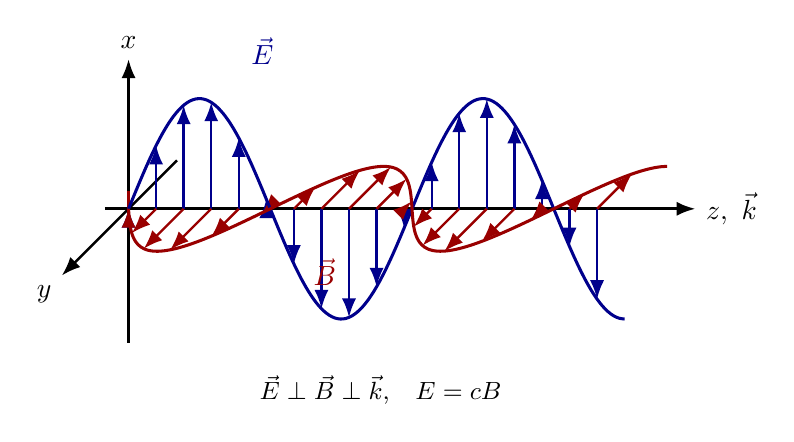
\begin{tikzpicture}[line width=0.85pt,>={Latex[length=2.4mm]}]
  \draw[->,line width=1pt] (-0.3,0,0)--(7.2,0,0) node[right]{$z,\ \vec k$};
  \draw[->] (0,-1.7,0)--(0,1.9,0) node[above]{$x$};
  \draw[->] (0,0,-1.6)--(0,0,2.2) node[below left]{$y$};
  % E (vertical, azul) y B (perspectiva y, rojo)
  \foreach \z in {0,0.35,...,6.3}{
    \pgfmathsetmacro{\a}{1.4*sin(\z*100)}
    \draw[blue!55!black,->] (\z,0,0)--(\z,\a,0);
    \draw[red!60!black,->] (\z,0,0)--(\z,0,\a);
  }
  \draw[blue!55!black,line width=1.1pt,domain=0:6.3,samples=90,smooth,variable=\z] plot (\z,{1.4*sin(\z*100)},0);
  \draw[red!60!black,line width=1.1pt,domain=0:6.3,samples=90,smooth,variable=\z] plot (\z,0,{1.4*sin(\z*100)});
  \node[blue!55!black] at (1.7,2.0){$\vec E$};
  \node[red!60!black] at (3.3,0,2.1){$\vec B$};
  \node at (3.2,-2.3){\small $\vec E\perp\vec B\perp\vec k$,\quad $E=cB$};
\end{tikzpicture}
\end{document}
